
%        File: WeeklyResearchReport_4_19_21.tex
%     Created: Mon Apr 19 08:00 AM 2021 E
% Last Change: Mon Apr 19 08:00 AM 2021 E
%
\documentclass[a4paper]{article}
\usepackage{mathtools}
\usepackage{verbatim}
\usepackage{graphicx}
\usepackage{tabularx}
\usepackage{pgfplots}
\usepackage{adjustbox}
\usepackage{booktabs}
\makeatletter
\let\latex@xfloat=\@xfloat
\def\@xfloat #1[#2]{%
    \latex@xfloat #1[#2]%
    \def\baselinestretch{1}
    \@normalsize\normalsize
    \normalsize
}
\makeatother
\usepackage{amsmath}
\usepackage{mathtools}
\usepackage{epigraph}
\usepackage{cancel}
\usepackage{xcolor}
\newcommand\Ccancel[2][black]{\renewcommand\CancelColor{\color{#1}}\cancel{#2}}
\usepackage{algorithm}
\usepackage{graphicx}
\usepackage[noend]{algpseudocode}
\usepackage{gnuplot-lua-tikz}
\usepackage[utf8]{inputenc}
\usepackage{pgfplots}
\usepackage{tabularx}
\DeclareUnicodeCharacter{2212}{−}
\usepgfplotslibrary{groupplots,dateplot}
\usetikzlibrary{patterns,shapes.arrows}
\pgfplotsset{compat=newest}
\begin{document}
\begin{titlepage}

    \title{
    Daily Research Report}

    \author{ Jeffrey Severino \\
        University of Toledo \\
        Toledo, OH  43606 \\
    email: jseveri@rockets.utoledo.edu}


    \maketitle

\end{titlepage}
\section{Current Research Direction}
The goal is to analyze the data from SWIRL so that I have all the data I need this week. 
I am doing a prelimary results section to see if I am documenting my results properly.
\section{Research Performed}
The MMS was used to determine the asymptotic rates of convergence for the numerical
integration and for the LEE which contain radial derivative. The results show 
a series of grids starting with 7 grid points and doubling with each iteration.
After seven iterations the numerical integration method was converged to second
order accuracy. After nine iterations the LEE ROC was 1.956908751121.  

A series of hyperbolic tangents were used to obtain a mean flow profile with
significant slope changes at various locations along the radial grid. The same 
method was used to obtain the manufactured expressions for the perturbation variables
Figure 2 shows the expected vs actual speed of sound obtained from SWIRL. Figure 3
shows the gradual decrease in error for the first 3 grids used for the speed of sound.
The same first three grids were used as demonstration for the LEE.  

The source terms show what is keeping the code from converging. Note that the locations
where there is a steep gradient, there is a lot of change from grid to grid 
at low grid points. The reason for this is that Second order differencing needs
a high number of grid points to resolve numerical approximations around large derivative 
values. Note that $S_4$ converges relatively quickly but also lacks the large gradient
changes.
 \begin{figure}
     \centering
     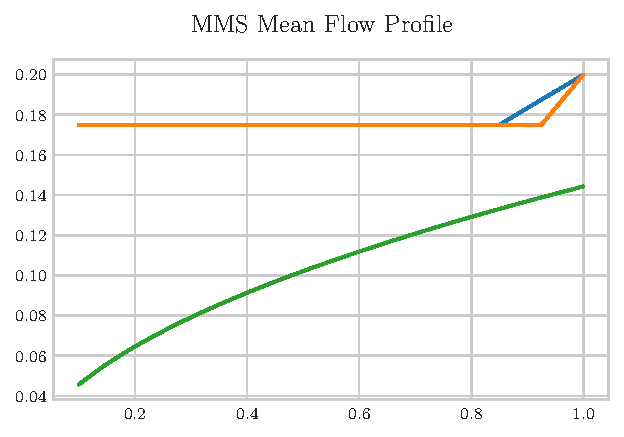
\includegraphics[width=\textwidth]{/home/jeff-severino/SWIRL/CodeRun/03-plotReport/tex-outputs/MMS_meanFlow.pdf}
     \caption{Mean Flow Profile for the Manufactured Solution Test}
 \end{figure}



 \begin{figure}
     \centering
     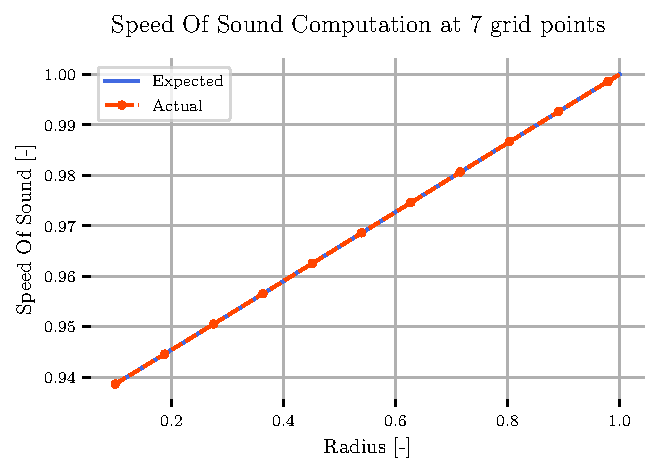
\includegraphics[width=\textwidth]{/home/jeff-severino/SWIRL/CodeRun/03-plotReport/tex-outputs/SpeedOfSoundComparison1.pdf}
     \caption{Expected vs Actual Speed of Sound}
 \end{figure}

 \begin{figure}
     \centering
     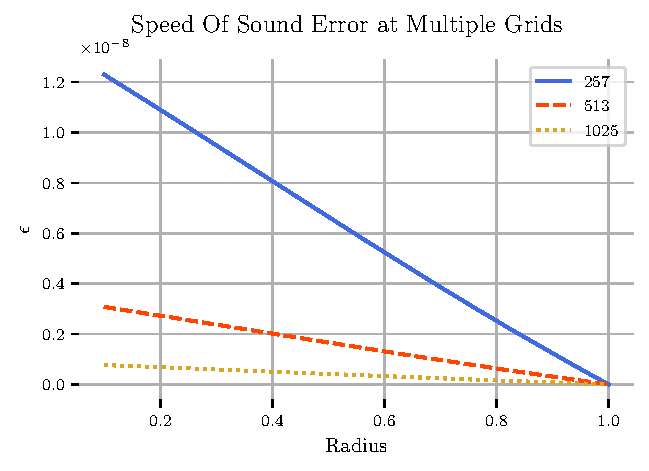
\includegraphics[width=\textwidth]{/home/jeff-severino/SWIRL/CodeRun/03-plotReport/tex-outputs/SpeedOfSoundComparison2.pdf}
     \caption{Speed of Sound Error}
 \end{figure}


 \begin{figure}
     \centering
     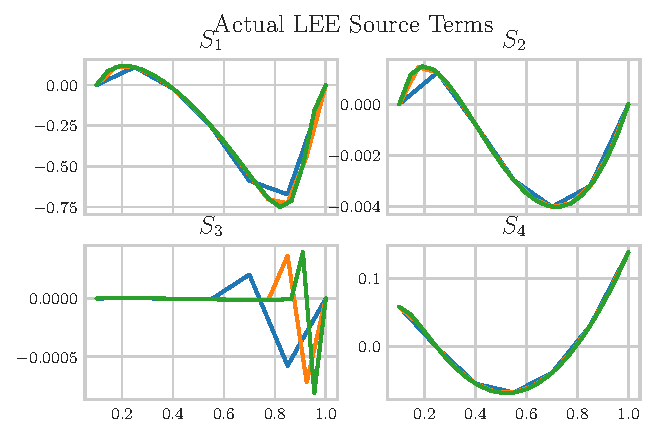
\includegraphics[width=\textwidth]{/home/jeff-severino/SWIRL/CodeRun/03-plotReport/tex-outputs/SourceTermActual.pdf}
     \caption{Actual LEE Source terms for the first 3 grids}
 \end{figure}

 \begin{figure}
     \centering
     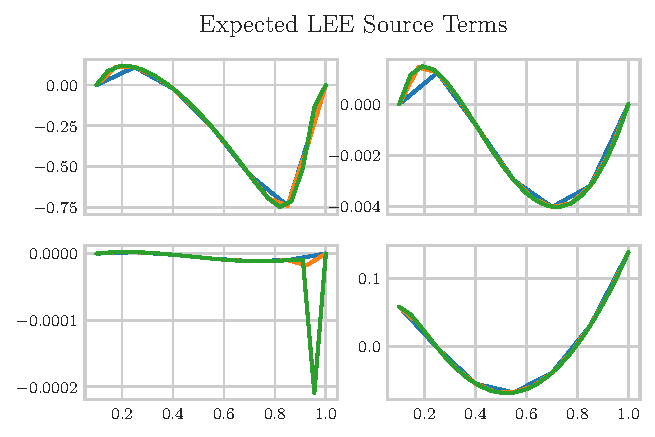
\includegraphics[width=\textwidth]{/home/jeff-severino/SWIRL/CodeRun/03-plotReport/tex-outputs/SourceTermExpected.pdf}
     \caption{Expected LEE Source terms for the first 3 grids}
 \end{figure}


 \begin{figure}
     \centering
     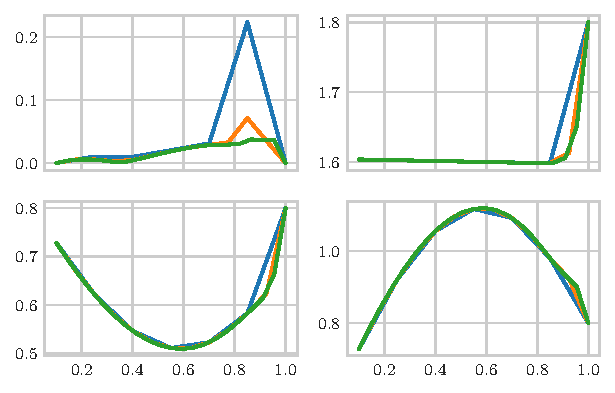
\includegraphics[width=\textwidth]{/home/jeff-severino/SWIRL/CodeRun/03-plotReport/tex-outputs/SourceTermError.pdf}
     \caption{Source Term Error}
 \end{figure}



 \begin{figure}
     \centering
     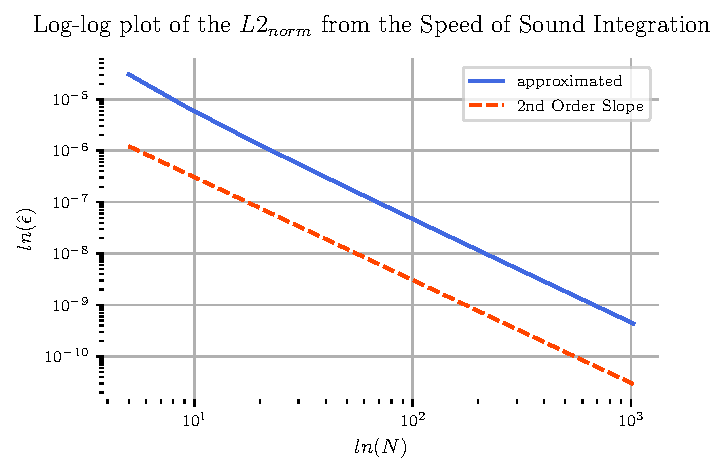
\includegraphics[width=\textwidth]{/home/jeff-severino/SWIRL/CodeRun/03-plotReport/tex-outputs/SND_L2.pdf}
     \caption{Speed of Sound L2}
 \end{figure}


 \begin{figure}
     \centering
     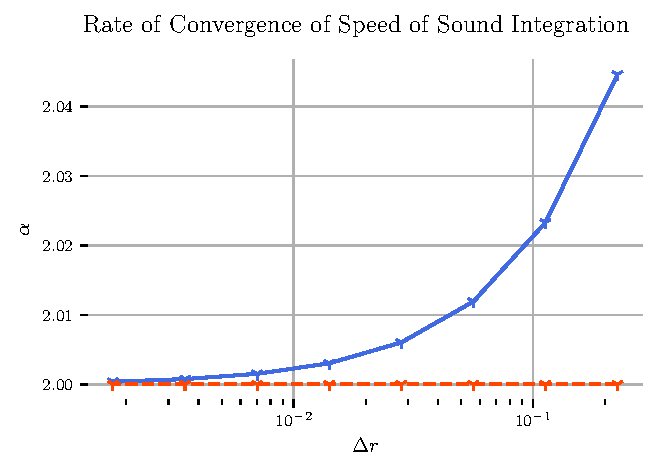
\includegraphics[width=\textwidth]{/home/jeff-severino/SWIRL/CodeRun/03-plotReport/tex-outputs/SND_ROC.pdf}
     \caption{Speed of Sound ROC}
 \end{figure}


 \begin{figure}
     \centering
     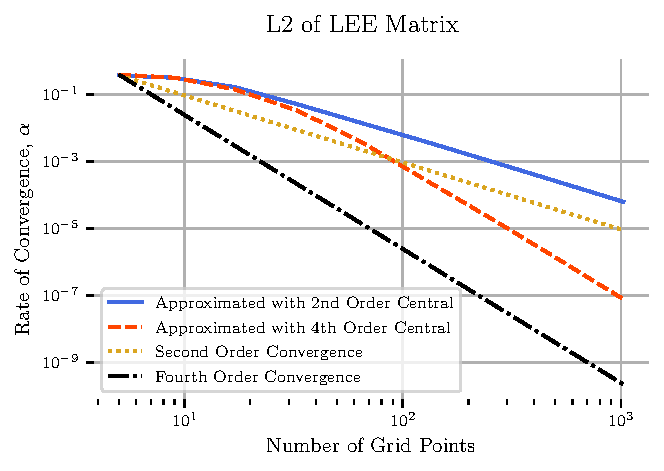
\includegraphics[width=\textwidth]{/home/jeff-severino/SWIRL/CodeRun/03-plotReport/tex-outputs/LEE_L2.pdf}
     \caption{LEE L2}
 \end{figure}


 \begin{figure}
     \centering
     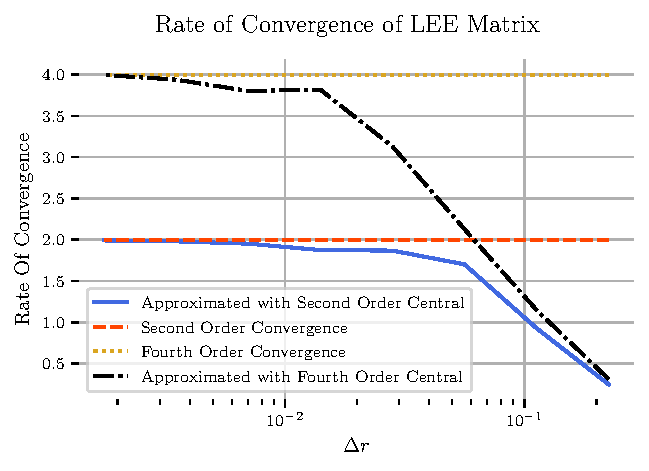
\includegraphics[width=\textwidth]{/home/jeff-severino/SWIRL/CodeRun/03-plotReport/tex-outputs/LEE_ROC.pdf}
     \caption{LEE ROC}
 \end{figure}




\section{Issues and Concerns}
I should super impose the fourth order results for the final number of grid points 
chosen.
\section{Planned Research}

\end{document}


